\section{Virtualization technologies}
\label{sec:leavingvirtualization}

A broad, loose, and multiple-purpose oriented definition of (computer) virtualization can be taken out of the excellent essay that is~\cite{introvirtualization}:
\begin{displayquote}
Virtualization is a framework or methodology of dividing the resources of a computer into multiple execution environments, by applying one or more concepts or technologies such as hardware and software partitioning, time-sharing, partial or complete machine simulation, emulation, quality of service, and many others.
\end{displayquote}

However, to narrow down the definition in this case, we can say that a virtual machine, on a modern multiprocess operating system, is a \emph{context} where created by the means of software, one or more programs can be running in isolation from the outside of that context.

The degree by which this isolation is provided varies on different kinds of virtualization.

For example, VMware Workstation (and free alternatives to it, such as VirtualBox by Sun, now Oracle) allows a full operating system to be installed on a virtual disk, which consists in one or more files stored in a place, local or remote, to where the host machine's OS has access, and implements abstractions for hardware components such as NICs, other virtual hard disks, and video cards, limits the amount of the host's memory and CPU cores which can be used from and by the VM---the guest. % TODO NICs on the gls
Such a system is what we refer to as ``full blown virtualization,'' or simply a virtual machine (VM).
A solution like this one, in practice, demands the the resources necessary for a working machine (including its operating system, drivers, background processes, etc.) are provided by each VM that is a guest on a given host, since there isn't any sharing of some of that ``burden.''

Nowadays, desktop operating systems like Linux-based ones, macOS, or Microsoft Windows provide hypervisors that allow to create full-blown virtual machines with a lower overhead since the hardware abstractions are in the kernel or closer to it.
For these operating systems, those technologies are, respectively, KVM, Apple's Hypervisor, and Hyper-V~\cite{whatiskvm,applehypervisor,hyperv}.

As~\cite{introvirtualization} describes, full virtual machines was typically a costly thing to do, especially on x86-based machines.
However, the article is question is quite old.
Even though there are more lightweight alternatives, presented afterwards, full-blown virtual machines are nowadays lighter, modern x86 processors provide hardware acceleration techniques to make it closer to native as well, and the sheer capacity of commodity hardware is also bigger than ever~\cite{virtualizationcontainerization}.

However, other solutions exist that provide lower isolation levels (from an implementation standpoint) that can suffice for certain applications, as shown in later chapters. Nowadays, this concept is usually called containers.
A container is a process running on the host's OS which resorts to technologies like \emph{Cgroups} and \emph{namespaces}, both provided by the Linux kernel, to be able to isolate its child processes from the host's or other containers' processes, namely in aspects of networking.
However, the kernel is actually the same, which reduces the overhead dramatically~\cite{comparativevmscontainers}.

A particular container infrastructure, very popular nowadays is Docker, which uses the aforementioned Linux kernel technologies but provides a whole set of tools that make working with containers, pre-defining \emph{images} to run on containerized infrastructure and distributing them, configuring, and even transparently providing a thin Linux virtual machine for non-Linux desktop environments.

A high-level illustration of the difference between applications running on ``regular,'' full-blown VMs and applications running over Docker (here, Docker represents the full set of OS-functionality and APIs it abstracts to provide a ``container infrastructure'') is offered by figure~\ref{fig:docker-vs-vms}, taken from~\cite{dockercontreplacingvms}.

% Figure fig:docker-vs-vms
\begin{figure}
  \centering
  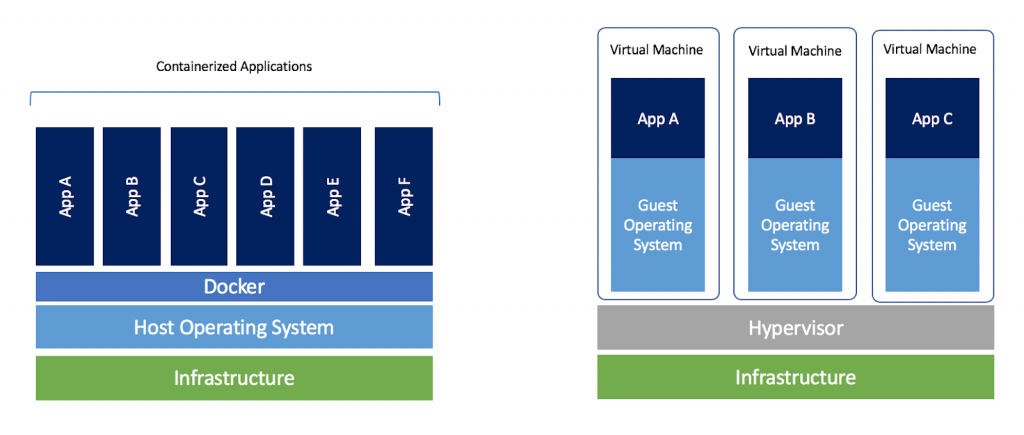
\includegraphics[width=0.8\textwidth]{docker-vs-vms}
  \caption{\textquote{Containers versus Virtual Machines}}
  \label{fig:docker-vs-vms}
\end{figure}



% end of section leavingvirtualizationtechnologies
